\chapter{Daur Hidup dan Perkembangbiakan Tumbuhan Darat}\label{ch:b2:plant-life-cycles}

Bantalan hijau \omterm{def:b2:plant-life-cycles:moss}{lumut} pada sebuah dinding adalah satu tumbuhan; tangkai
cokelat yang menjulang darinya pada musim semi, masing-masing dengan
sebuah kapsul berisi spora, adalah tumbuhan lain --- individu yang
berbeda, dengan kromosom dua kali lipat, tumbuh dari yang pertama dan
hidup di atasnya. Sehelai ental \omterm{def:b2:plant-life-cycles:fern}{tumbuhan paku} mengusung spora di sisi
bawahnya, tetapi sporanya tidak tumbuh menjadi \omterm{def:b2:plant-life-cycles:fern}{tumbuhan paku}: sporanya
tumbuh menjadi sisik hijau berbentuk jantung selebar beberapa
milimeter, dan di situlah sperma serta sel telurnya dibuat, dan dari
sisik itulah sebatang \omterm{def:b2:plant-life-cycles:fern}{tumbuhan paku} baru muncul. Tiap tumbuhan darat
bergiliran dengan cara ini antara dua tubuh, satu \omterm{def:b2:meiosis-heredity:meiosis}{haploid} dan satu
\omterm{def:b2:meiosis-heredity:meiosis}{diploid}. Bab ini mengikuti pergiliran itu dari alga sampai ke biji, dan
menunjukkan bagaimana serangkaian perubahan padanya --- penyusutan
tubuh \omterm{def:b2:meiosis-heredity:meiosis}{haploidnya}, penemuan \omterm{def:b2:plant-life-cycles:heterospory}{serbuk sari}, pengurungan \omterm{def:b2:plant-life-cycles:heterospory}{bakal biji}, dan
bijinya --- membebaskan perkembangbiakan dari air lalu membiarkan
tumbuhan menutupi benua.

\section{Tiga macam daur hidup}

\begin{definition}[Haplontik, diplontik, haplo-diplontik]\label{def:b2:plant-life-cycles:cycles}
\index{daur hidup}\index{pergiliran keturunan}\index{gametofit}\index{sporofit}
Tiap daur hidup seksual memuat satu \emph{pembuahan}, yang
melipatduakan cacah kromosomnya, dan satu \emph{\omterm{def:b2:meiosis-heredity:meiosis}{meiosis}}, yang
memerohkannya; daurnya berbeda dalam apa yang terjadi di antara
keduanya. Pada daur \emph{haplontik}, zigotnya adalah satu-satunya sel
\omterm{def:b2:meiosis-heredity:meiosis}{diploid} dan langsung menjalani \omterm{def:b2:meiosis-heredity:meiosis}{meiosis}; organismenya \omterm{def:b2:meiosis-heredity:meiosis}{haploid} dan
gametnya dibuat secara mitosis (\emph{Chlamydomonas}, banyak alga dan
fungi). Pada daur \emph{diplontik}, \omterm{def:b2:meiosis-heredity:meiosis}{meiosis} membuat gamet secara
langsung, gametnya adalah satu-satunya sel \omterm{def:b2:meiosis-heredity:meiosis}{haploid}, dan organismenya
\omterm{def:b2:meiosis-heredity:meiosis}{diploid} (hewan, alga cokelat \emph{Fucus}). Pada daur
\emph{haplo-diplontik}, \omterm{def:b2:meiosis-heredity:meiosis}{meiosis} membuat \emph{spora}, yang tumbuh
secara mitosis menjadi organisme \omterm{def:b2:meiosis-heredity:meiosis}{haploid}, yaitu \emph{gametofit}, yang
membuat gamet secara mitosis; zigotnya tumbuh secara mitosis menjadi
organisme \omterm{def:b2:meiosis-heredity:meiosis}{diploid}, yaitu \emph{sporofit}, yang membuat spora secara
\omterm{def:b2:meiosis-heredity:meiosis}{meiosis}. Dua tubuh \omterm{def:b2:unicellular-diversity:unicellular}{bersel banyak} bergiliran --- itulah
\emph{pergiliran keturunan} --- dan inilah daur tiap tumbuhan darat
dan banyak alga.
\end{definition}

\begin{omfigure}
\begin{tikzpicture}[every node/.style={font=\scriptsize}, >=stealth]
  \foreach \dx/\title/\hap/\dip in {0/{haplontik (\emph{Chlamydomonas})}/{organisme haploid ($n$)}/{zigot ($2n$)}, 5.2/{diplontik (hewan)}/{gamet ($n$)}/{organisme diploid ($2n$)}, 10.4/{haplo-diplontik (tumbuhan)}/{gametofit ($n$)}/{sporofit ($2n$)}} {
    \begin{scope}[xshift=\dx cm]
      \node[anchor=south, font=\scriptsize\bfseries] at (2,2.5) {\title};
      \draw[thick, omDef, ->] (0.6,0.4) arc (200:340:1.5 and 1.0);
      \draw[thick, omThm, ->] (3.4,1.4) arc (20:160:1.5 and 1.0);
      \node[omDef, anchor=north] at (2,-0.3) {\hap};
      \node[omThm, anchor=south] at (2,2.05) {\dip};
      \node[anchor=south west] at (3.4,1.05) {pembuahan};
      \node[anchor=north east] at (0.55,0.75) {meiosis};
    \end{scope}
  }
  % emphasise the dominant phase by thickness of the arcs: draw thicker arcs
  \draw[line width=2.4pt, omDef, ->] (0.6,0.4) arc (200:340:1.5 and 1.0);
  \draw[line width=2.4pt, omThm, ->] (5.2+3.4,1.4) arc (20:160:1.5 and 1.0);
  \draw[line width=2.4pt, omDef, ->] (10.4+0.6,0.4) arc (200:340:1.5 and 1.0);
  \draw[line width=2.4pt, omThm, ->] (10.4+3.4,1.4) arc (20:160:1.5 and 1.0);
\end{tikzpicture}

{\small Tiga \omterm{def:b2:plant-life-cycles:cycles}{daur hidup}. Biru: fase \omterm{def:b2:meiosis-heredity:meiosis}{haploidnya}; merah: fase
\omterm{def:b2:meiosis-heredity:meiosis}{diploidnya}; busur yang tebal adalah tubuh \omterm{def:b2:unicellular-diversity:unicellular}{bersel banyaknya}. Tiap
daurnya melewati \omterm{def:b2:meiosis-heredity:meiosis}{meiosis} sekali dan pembuahan sekali; yang membedakan
adalah fase mana --- atau keduanya --- yang tumbuh menjadi organisme.}
\end{omfigure}

\begin{proposition}[Apa arti pergiliran keturunan]\label{prop:b2:plant-life-cycles:alternation}
Pada tumbuhan darat, kedua keturunannya adalah dua organisme, bukan dua
tahap satu organisme: \omterm{def:b2:plant-life-cycles:cycles}{gametofit} dan \omterm{def:b2:plant-life-cycles:cycles}{sporofitnya} memiliki genom yang
berbeda (\omterm{def:b2:meiosis-heredity:meiosis}{haploid} dan \omterm{def:b2:meiosis-heredity:meiosis}{diploid}), tubuh yang berbeda, kerap ukuran yang
berbeda sampai beberapa orde besar, dan masing-masing berkembang
secara mitosis dari satu sel --- sebuah spora atau sebuah zigot.
\omterm{def:b2:plant-life-cycles:cycles}{Gametofitnya} membuat gamet di dalam organ \omterm{def:b2:unicellular-diversity:unicellular}{bersel banyak}, yaitu
\emph{\omterm{def:b2:plant-life-cycles:moss}{anteridium}} (sperma) dan \emph{\omterm{def:b2:plant-life-cycles:moss}{arkegonium}} (masing-masing satu
sel telur, di dalam labu yang lehernya direnangi spermanya ke bawah);
\omterm{def:b2:plant-life-cycles:cycles}{sporofitnya} membuat spora di dalam \emph{\omterm{def:b2:plant-life-cycles:fern}{sporangium}}. Menyeberangi
tumbuhan darat, keseimbangannya bergeser: pada \omterm{def:b2:plant-life-cycles:moss}{lumut}, \omterm{def:b2:plant-life-cycles:cycles}{gametofitnya}
adalah tumbuhannya dan \omterm{def:b2:plant-life-cycles:cycles}{sporofitnya} sebuah tangkai yang bergantung
padanya; pada \omterm{def:b2:plant-life-cycles:fern}{tumbuhan paku}, \omterm{def:b2:plant-life-cycles:cycles}{sporofitnya} adalah tumbuhannya dan
\omterm{def:b2:plant-life-cycles:cycles}{gametofitnya} sebuah sisik yang hidup bebas; pada tumbuhan berbiji,
\omterm{def:b2:plant-life-cycles:cycles}{gametofitnya} menyusut menjadi beberapa sel yang tersembunyi di dalam
jaringan \omterm{def:b2:plant-life-cycles:cycles}{sporofitnya} --- yaitu butir \omterm{def:b2:plant-life-cycles:heterospory}{serbuk sari} dan isi \omterm{def:b2:plant-life-cycles:heterospory}{bakal bijinya}.
\end{proposition}
\begin{proof}[Bukti eksperimental]
Hofmeister (1851) mengecambahkan spora \omterm{def:b2:plant-life-cycles:moss}{lumut}, \omterm{def:b2:plant-life-cycles:fern}{tumbuhan paku}, paku ekor
kuda, dan paku kawat, mengikuti perkembangan tubuh hijau kecil yang
dihasilkannya, mendapati \omterm{def:b2:plant-life-cycles:moss}{anteridium} dan \omterm{def:b2:plant-life-cycles:moss}{arkegonium} padanya, lalu
menyaksikan lembaganya tumbuh dari sel telur yang telah dibuahi di
dalam \omterm{def:b2:plant-life-cycles:moss}{arkegoniumnya} menjadi tumbuhan pengusung spora. Ia lalu
menunjukkan bahwa \omterm{def:b2:plant-life-cycles:heterospory}{bakal biji} sebatang konifer memuat struktur yang
sama, dalam bentuk yang menyusut --- \omterm{def:b2:plant-life-cycles:moss}{arkegonium} di dalam jaringan yang
merupakan \omterm{def:b2:plant-life-cycles:cycles}{gametofit} yang ditahan --- dan bahwa dengan demikian \omterm{def:b2:plant-life-cycles:moss}{lumut},
\omterm{def:b2:plant-life-cycles:fern}{tumbuhan paku}, dan tumbuhan berbiji adalah satu deret dengan satu daur.
Cacah kromosom yang menjelaskan kedua keturunannya (Strasburger, 1894)
baru datang empat puluh tahun kemudian.
\end{proof}

\section{Lumut: gametofitnya adalah tumbuhannya}

\begin{definition}[Daur hidup lumut]\label{def:b2:plant-life-cycles:moss}
\index{lumut}\index{protonema}\index{arkegonium}\index{anteridium}
Sebuah \emph{spora} lumut berkecambah menjadi filamen hijau bercabang,
yaitu \emph{protonema}, yang darinya tunas tumbuh menjadi pucuk berdaun
--- \emph{\omterm{def:b2:plant-life-cycles:cycles}{gametofit}}, setinggi beberapa sentimeter, tanpa akar sejati,
tanpa xilem maupun floem, ditambatkan rizoid dan menyerap air lewat
seluruh permukaannya. Pada ujung pucuknya ia mengusung
\emph{anteridium}, yang melepaskan sperma berflagelum dua ke dalam
selaput air hujan atau embun, dan \emph{arkegonium}, yang masing-masing
berisi satu sel telur di dasar sebuah leher; spermanya berenang paling
jauh beberapa sentimeter, dituntun zat penarik kimia, lalu membuahi sel
telurnya di tempat. Zigotnya tumbuh menjadi \emph{\omterm{def:b2:plant-life-cycles:cycles}{sporofit}}: sebuah
kaki yang terbenam di dalam \omterm{def:b2:plant-life-cycles:cycles}{gametofitnya}, sebuah tangkai (\emph{seta}),
dan sebuah \emph{kapsul} yang di dalamnya \omterm{def:b2:meiosis-heredity:meiosis}{meiosis} membuat puluhan ribu
spora, yang dilepaskan lewat cincin gigi higroskopik yang membuka di
udara kering. \omterm{def:b2:plant-life-cycles:cycles}{Sporofitnya} berfotosintesis sedikit tetapi disuapi
\omterm{def:b2:plant-life-cycles:cycles}{gametofitnya} lewat kakinya dan tidak pernah hidup sendiri.
\end{definition}

\begin{omfigure}
\begin{tikzpicture}[every node/.style={font=\scriptsize}, >=stealth]
  \node[draw, rounded corners, fill=omDef!12, align=center] (spore) at (0,3) {spora ($n$)};
  \node[draw, rounded corners, fill=omDef!12, align=center] (proto) at (3.2,3) {protonema};
  \node[draw, rounded corners, fill=omDef!12, align=center] (gam) at (6.6,3) {gametofit berdaun ($n$)\\anteridium dan arkegonium};
  \node[draw, rounded corners, fill=omDef!12, align=center] (gametes) at (11.2,3) {sperma dan sel telur ($n$)};
  \node[draw, rounded corners, fill=omThm!12, align=center] (zyg) at (11.2,0.8) {zigot ($2n$)};
  \node[draw, rounded corners, fill=omThm!12, align=center] (sporo) at (6.6,0.8) {sporofit ($2n$)\\kaki, seta, kapsul};
  \node[draw, rounded corners, fill=omThm!12, align=center] (cap) at (2.4,0.8) {meiosis di dalam kapsulnya};
  \draw[->, thick] (spore) -- (proto) node[midway, above] {mitosis};
  \draw[->, thick] (proto) -- (gam);
  \draw[->, thick] (gam) -- (gametes) node[midway, above] {mitosis};
  \draw[->, thick] (gametes) -- (zyg) node[pos=0.3, right, align=left] {pembuahan\\di dalam selaput air};
  \draw[->, thick] (zyg) -- (sporo) node[midway, above] {mitosis};
  \draw[->, thick] (sporo) -- (cap);
  \draw[->, thick] (cap) -| (spore) ;
  \node[omDef, anchor=west] at (-1.9,3.9) {haploid};
  \node[omThm, anchor=west] at (-1.9,-0.1) {diploid};
  \draw[gray, dashed] (-1.9,1.9) -- (13.2,1.9);
\end{tikzpicture}

{\small Daur \omterm{def:b2:plant-life-cycles:moss}{lumut}. Tumbuhan berdaunnya adalah \omterm{def:b2:plant-life-cycles:cycles}{gametofit} yang
\omterm{def:b2:meiosis-heredity:meiosis}{haploid}; \omterm{def:b2:plant-life-cycles:cycles}{sporofitnya} adalah tangkai dan kapsul yang tumbuh di atasnya,
disuapi olehnya, dan membuat spora secara \omterm{def:b2:meiosis-heredity:meiosis}{meiosis}.}
\end{omfigure}

\begin{omfigure}
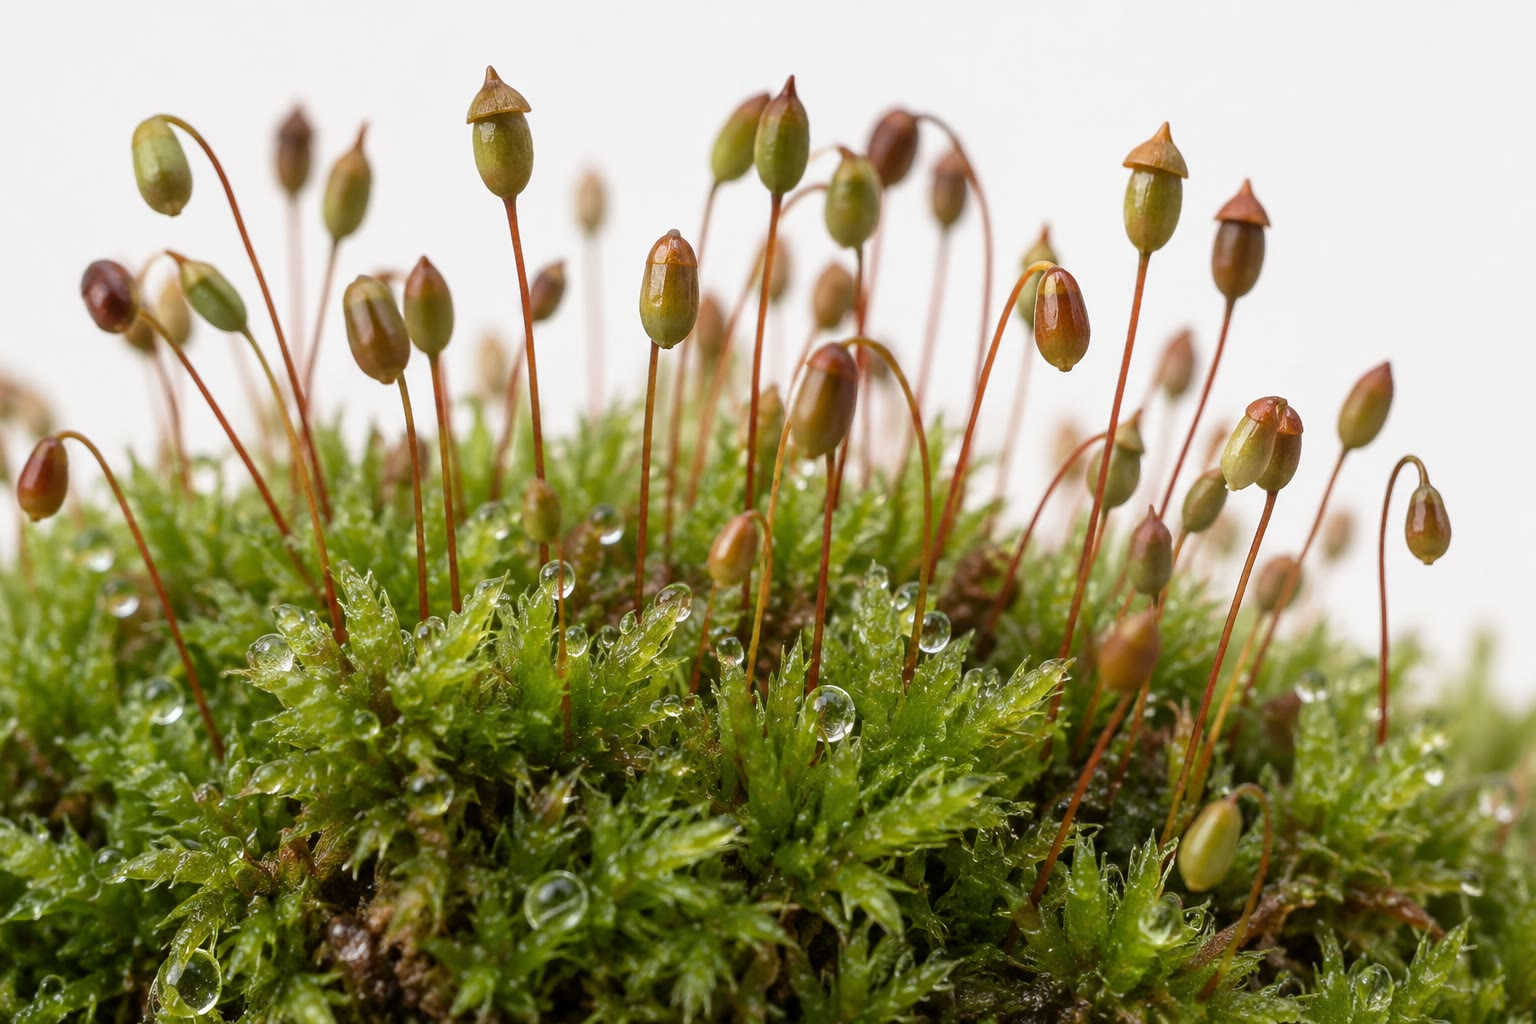
\includegraphics[width=0.6\linewidth]{images/book4/ai/b4-05-moss-sporophytes.jpg}

{\small Bantalan \omterm{def:b2:plant-life-cycles:moss}{lumut} pada musim semi: pucuk hijaunya adalah
\omterm{def:b2:plant-life-cycles:cycles}{gametofitnya}, dan tiap tangkai kemerahan dengan kapsulnya adalah sebuah
\omterm{def:b2:plant-life-cycles:cycles}{sporofit} yang tumbuh dari sel telur yang telah dibuahi, masih melekat
pada pucuk yang membuat sel telur itu.}
\end{omfigure}

\begin{example}[Ongkos sperma yang berenang]\label{ex:b2:plant-life-cycles:sperm}
Sperma \omterm{def:b2:plant-life-cycles:moss}{lumut} berenang pada kira-kira \qty{100}{\micro m/s}; untuk
mencapai sebuah \omterm{def:b2:plant-life-cycles:moss}{arkegonium} sejauh \qty{2}{cm} ia membutuhkan
\qty{200}{s} selaput air yang sinambung --- sepercik hujan, embun yang
tebal. Maka pembuahannya terbatas pada cuaca yang basah dan pada jarak
yang pendek, dan sebagian besar \omterm{def:b2:plant-life-cycles:moss}{lumut}, \omterm{def:b2:plant-life-cycles:fern}{tumbuhan paku}, serta kerabatnya
hidup di tempat lembap atau berbiak pada musim hujan; \omterm{def:b2:plant-life-cycles:moss}{anteridium}
sebagian \omterm{def:b2:plant-life-cycles:moss}{lumut} duduk di dalam cawan percik yang bentuknya melontarkan
tetes hujan, beserta sperma yang diusungnya, sejauh setengah meter.
Ketergantungan inilah yang dilepaskan tumbuhan berbiji.
\end{example}

\section{Tumbuhan paku: sporofitnya adalah tumbuhannya}

\begin{definition}[Daur hidup tumbuhan paku]\label{def:b2:plant-life-cycles:fern}
\index{tumbuhan paku}\index{protalus}\index{sorus}\index{sporangium}
Tumbuhan pakunya adalah \emph{\omterm{def:b2:plant-life-cycles:cycles}{sporofit}}: sebuah rimpang berakar,
berxilem, dan berfloem, serta berental. Pada sisi bawah ental yang
subur, gerombolan \emph{sporangium} (\emph{sorus}, kerap di bawah
sebuah tudung pelindung) masing-masing membuat 64 spora secara \omterm{def:b2:meiosis-heredity:meiosis}{meiosis}
lalu melontarkannya lewat sentakan cincin sel berdinding tebal yang
mengering. Sebuah spora yang mendarat di tanah lembap tumbuh menjadi
sebuah \emph{protalus}: \omterm{def:b2:plant-life-cycles:cycles}{gametofit} hijau berbentuk jantung selebar
beberapa milimeter, setebal satu sel, berizoid, dan hidup bebas selama
beberapa pekan. Ia mengusung \omterm{def:b2:plant-life-cycles:moss}{anteridium} dan \omterm{def:b2:plant-life-cycles:moss}{arkegonium} pada sisi
bawahnya; spermanya berenang di dalam selaput air tanah menuju sel
telurnya; zigotnya tumbuh menjadi \omterm{def:b2:plant-life-cycles:cycles}{sporofit} muda yang menarik makanan
pertamanya dari protalusnya lalu berakar, dan protalusnya mati. Kedua
keturunannya sama-sama merdeka, tetapi tidak setara: \omterm{def:b2:plant-life-cycles:cycles}{sporofitnya} hidup
berpuluh tahun dan dapat setinggi beberapa meter, \omterm{def:b2:plant-life-cycles:cycles}{gametofitnya} hidup
beberapa pekan dan setinggi beberapa milimeter.
\end{definition}

\begin{omfigure}
\begin{tikzpicture}[every node/.style={font=\scriptsize}, >=stealth]
  \node[draw, rounded corners, fill=omThm!12, align=center] (fern) at (0,3) {tumbuhan paku, sang sporofit ($2n$)\\akar, rimpang, ental};
  \node[draw, rounded corners, fill=omThm!12, align=center] (sor) at (5.4,3) {sporangium di dalam sorus\\(di bawah entalnya)};
  \node[draw, rounded corners, fill=omDef!12, align=center] (spore) at (10.4,3) {spora ($n$)\\64 tiap sporangium};
  \node[draw, rounded corners, fill=omDef!12, align=center] (pro) at (10.4,0.6) {protalus ($n$)\\hidup bebas, berukuran mm\\anteridium, arkegonium};
  \node[draw, rounded corners, fill=omDef!12, align=center] (gam) at (5.4,0.6) {sperma dan sel telur ($n$)};
  \node[draw, rounded corners, fill=omThm!12, align=center] (zyg) at (0,0.6) {zigot ($2n$), lalu\\sporofit muda\\di atas protalusnya};
  \draw[->, thick] (fern) -- (sor);
  \draw[->, thick] (sor) -- (spore) node[midway, above] {meiosis};
  \draw[->, thick] (spore) -- (pro) node[midway, right] {mitosis};
  \draw[->, thick] (pro) -- (gam) node[midway, above] {mitosis};
  \draw[->, thick] (gam) -- (zyg) node[midway, above, align=center] {pembuahan\\(sperma berenang)};
  \draw[->, thick] (zyg) -- (fern) node[midway, right] {mitosis};
  \draw[gray, dashed] (7.9,-0.5) -- (7.9,4.0);
  \node[omThm, anchor=south] at (2.7,3.9) {keturunan diploid};
  \node[omDef, anchor=south] at (10.4,3.9) {keturunan haploid};
\end{tikzpicture}

{\small Daur \omterm{def:b2:plant-life-cycles:fern}{tumbuhan paku}. Tumbuhan yang kita sebut paku adalah
\omterm{def:b2:plant-life-cycles:cycles}{sporofit} yang \omterm{def:b2:meiosis-heredity:meiosis}{diploid}; \omterm{def:b2:plant-life-cycles:cycles}{gametofit} \omterm{def:b2:meiosis-heredity:meiosis}{haploidnya} adalah sebuah \omterm{def:b2:plant-life-cycles:fern}{protalus} yang
berumur pendek, dan di atasnya spermanya berenang menuju sel telurnya.}
\end{omfigure}

\begin{omfigure}
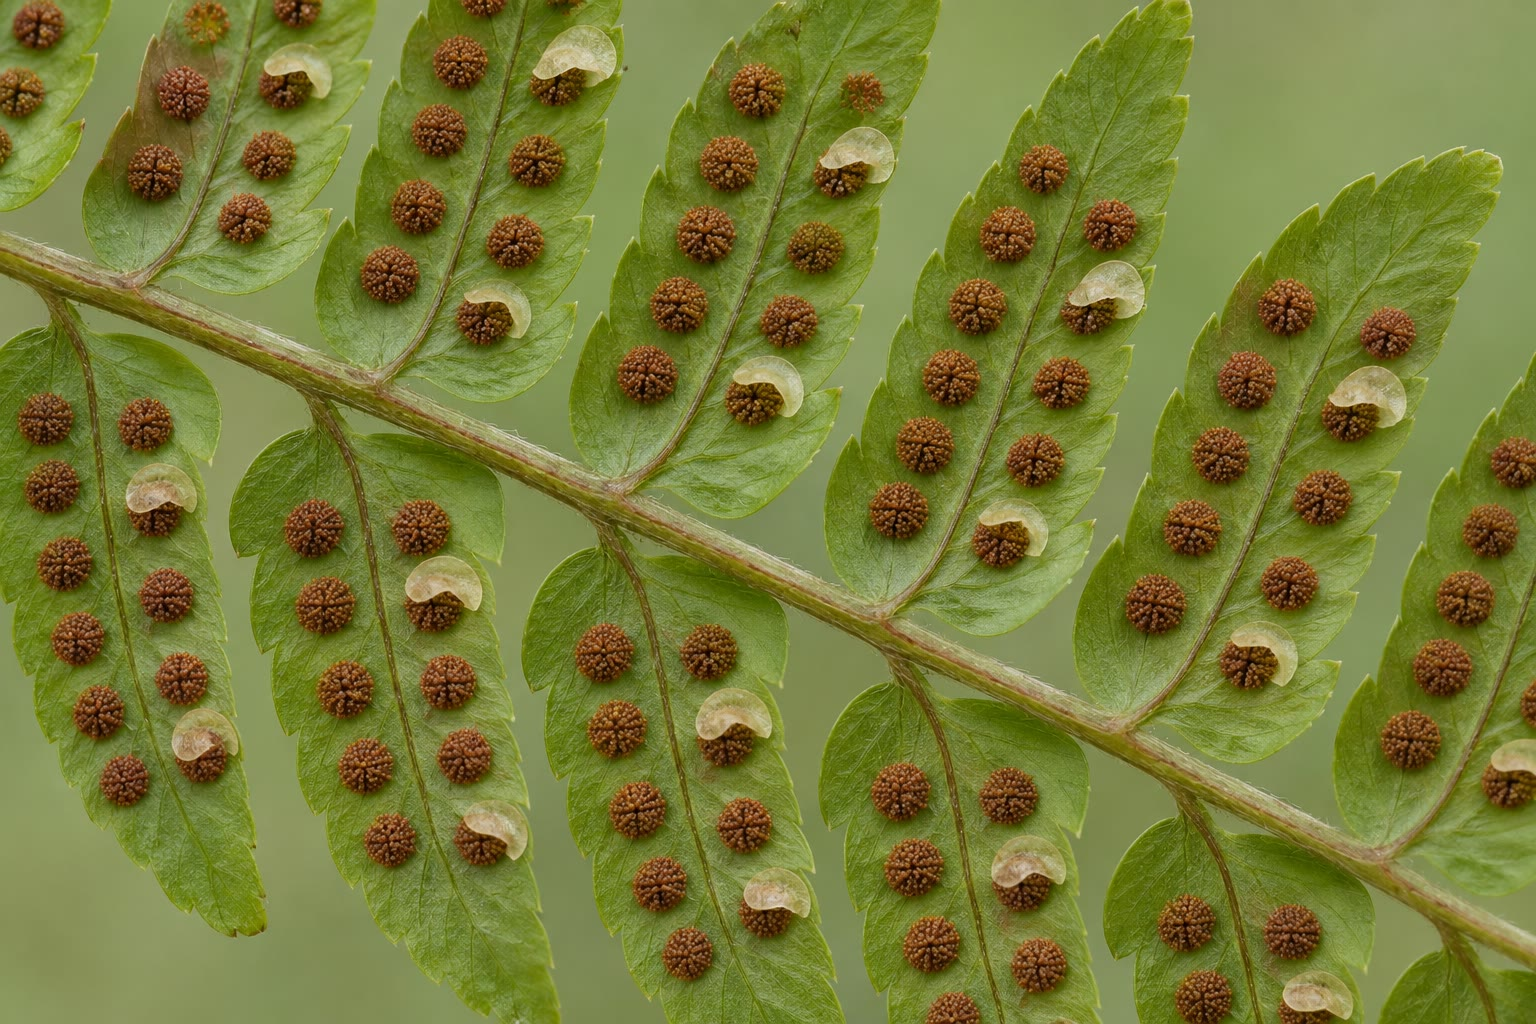
\includegraphics[width=0.6\linewidth]{images/book4/ai/b4-05-fern-sori.jpg}

{\small Sisi bawah sehelai ental paku yang subur: tiap bintik
cokelatnya adalah sebuah \omterm{def:b2:plant-life-cycles:fern}{sorus}, yaitu gerombolan \omterm{def:b2:plant-life-cycles:fern}{sporangium}, sebagian
masih tertutup tudung yang melindunginya sampai matang.}
\end{omfigure}

\begin{theorem}[Penyebaran sebuah spora]\label{thm:b2:plant-life-cycles:dispersal}
\index{penyebaran spora}
Sebuah spora berjari-jari $r$ dan bermassa jenis $\rho_s$ yang
dilepaskan pada ketinggian $h$ ke dalam angin mendatar berkelajuan $u$
jatuh pada kelajuan terminal Stokes
$v_s = 2r^2(\rho_s - \rho_{\text{udara}})g/9\eta_{\text{udara}}$
dan mendarat, di dalam udara yang berlapis tenang, pada jarak
\[
x = \frac{u\,h}{v_s}
\]
dari tumbuhannya. Sebuah spora paku berjari-jari \qty{15}{\micro m} dan
bermassa jenis \qty{1100}{kg/m^3} ($\eta_{\text{udara}} = \qty{1.8e-5}{Pa.s}$)
jatuh pada \qty{3}{cm/s}; dari sehelai ental pada \qty{0.5}{m} di dalam
angin \qty{2}{m/s} ia menempuh kira-kira \qty{30}{m}, dan di dalam
udara yang berolak pada hari berangin, yang mengangkat sebagian
sporanya jauh di atas ketinggian pelepasannya, beberapa spora menempuh
ratusan kilometer --- dan itulah sebabnya flora paku di pulau samudra
kaya sedangkan flora tumbuhan berbijinya miskin.
\end{theorem}
\begin{proof}
Waktu jatuhnya adalah $h/v_s$ (sporanya mencapai kelajuan terminalnya
dalam hitungan mikrodetik), dan selama itu anginnya membawanya sejauh
$u\,h/v_s$. Kelajuan terminalnya mengikuti dari penyeimbangan seretan
Stokes $6\pi\eta r
v_s$ terhadap beratnya dikurangi gaya apungnya $\tfrac43\pi r^3(\rho_s -
\rho_{\text{udara}})g$, seperti dalam \cref{ch:b2:unicellular-diversity}.
\end{proof}

\section{Tumbuhan berbiji: gametofitnya tersembunyi}

\begin{definition}[Heterospori, serbuk sari, bakal biji]\label{def:b2:plant-life-cycles:heterospory}
\index{heterospori}\index{serbuk sari}\index{bakal biji}\index{mikrospora}\index{megaspora}
\omterm{def:b2:plant-life-cycles:moss}{Lumut} dan sebagian besar \omterm{def:b2:plant-life-cycles:fern}{tumbuhan paku} bersifat \emph{homospor}: satu
macam spora, satu macam \omterm{def:b2:plant-life-cycles:cycles}{gametofit} yang mengusung kedua kelaminnya.
Tumbuhan berbiji (dan beberapa \omterm{def:b2:plant-life-cycles:fern}{tumbuhan paku} serta paku kawat)
bersifat \emph{heterospor}: \emph{mikrospora}, yang kecil dan banyak,
tumbuh menjadi \omterm{def:b2:plant-life-cycles:cycles}{gametofit} jantan; \emph{megaspora}, yang besar dan
sedikit, tumbuh menjadi \omterm{def:b2:plant-life-cycles:cycles}{gametofit} betina. Pada tumbuhan berbiji
keduanya menyusut menjadi hampir tiada dan tak satu pun meninggalkan
jaringan \omterm{def:b2:plant-life-cycles:cycles}{sporofitnya} sendirian. \omterm{def:b2:plant-life-cycles:cycles}{Gametofit} jantannya adalah \emph{butir
serbuk sari}: sebuah mikrospora yang telah membelah dua atau tiga kali
di dalam dindingnya, dibawa angin atau hewan menuju organ betinanya,
tempat ia menumbuhkan sebuah \emph{buluh serbuk sari} lalu
mengantarkan spermanya --- tanpa membutuhkan air. \omterm{def:b2:plant-life-cycles:cycles}{Gametofit} betinanya
berkembang di dalam megasporangiumnya, yang tinggal pada tetuanya
terkurung satu atau dua \emph{integumen} berliang, yaitu
\emph{mikropil}: seluruh strukturnya adalah \emph{bakal biji}. Sesudah
pembuahan, bakal bijinya menjadi \emph{biji}: sebuah lembaga \omterm{def:b2:plant-life-cycles:cycles}{sporofit},
sebuah simpanan makanan, dan sebuah kulit yang dibuat dari
integumennya, dorman sampai keadaannya tepat.
\end{definition}

\begin{omfigure}
\begin{tikzpicture}[every node/.style={font=\scriptsize}]
  % ovule in section
  \draw[thick, fill=omExo!25] (0,0) ellipse (1.6 and 2.2);
  \draw[thick, fill=omExo!10] (0,0) ellipse (1.25 and 1.85);
  \draw[thick, fill=white] (0,-0.15) ellipse (0.8 and 1.3);
  \draw[thick, fill=omDef!25] (0,0.6) ellipse (0.45 and 0.55);
  \fill[omDef!80!black] (0,0.75) circle (0.12);
  % micropyle: gap at top
  \fill[white] (-0.35,1.7) rectangle (0.35,2.35);
  \draw[thick] (-0.35,1.7) -- (-0.35,2.2); \draw[thick] (0.35,1.7) -- (0.35,2.2);
  \draw[thick] (-0.35,2.2) arc (180:90:0.1) ; \draw[thick] (0.35,2.2) arc (0:90:0.1);
  % pollen grain and tube
  \draw[thick, fill=omProp!40] (0.9,3.0) circle (0.22);
  \draw[thick, omProp] (0.75,2.85) .. controls (0.2,2.6) and (0.05,2.0) .. (0.05,1.25);
  % stalk
  \draw[thick] (0,-2.2) -- (0,-2.8);
  % labels
  \draw (1.45,-0.9) -- (2.6,-0.9) node[right] {integumen};
  \draw (1.0,-0.6) -- (2.6,-1.5) node[right] {megasporangium (nuselus)};
  \draw (0.55,-1.0) -- (2.6,-2.1) node[right, align=left] {gametofit betina\\(dari satu megaspora)};
  \draw (0.35,0.45) -- (2.6,0.3) node[right] {arkegonium};
  \draw (0.1,0.78) -- (2.6,1.0) node[right] {sel telur};
  \draw (0.35,2.0) -- (2.6,2.0) node[right] {mikropil};
  \draw (1.1,3.0) -- (2.6,3.0) node[right] {butir dan buluh serbuk sari};
  \node[right] at (0.1,-2.6) {tangkai};
\end{tikzpicture}

{\small Sebuah \omterm{def:b2:plant-life-cycles:heterospory}{bakal biji} gimnosperma dalam potongan. \omterm{def:b2:plant-life-cycles:cycles}{Gametofit}
betinanya, yang tumbuh dari satu \omterm{def:b2:plant-life-cycles:heterospory}{megaspora} di dalam megasporangiumnya,
terbungkus sebuah integumen berliang; butir \omterm{def:b2:plant-life-cycles:heterospory}{serbuk sarinya}, yang
tertangkap pada mikropilnya, menumbuhkan sebuah buluh menuju sel
telurnya. Sesudah pembuahan, seluruhnya menjadi bijinya.}
\end{omfigure}

\begin{proposition}[Daur konifer]\label{prop:b2:plant-life-cycles:conifer}
\index{konifer}\index{runjung}\index{biji}
Sebatang pinus mengusung dua macam runjung. \emph{Runjung jantan} yang
kecil, bergerombol pada musim semi, memuat mikrosporangium yang di
dalamnya \omterm{def:b2:meiosis-heredity:meiosis}{meiosis} membuat \omterm{def:b2:plant-life-cycles:heterospory}{mikrospora}; masing-masing membelah menjadi
butir \omterm{def:b2:plant-life-cycles:heterospory}{serbuk sari} berisi empat sel dengan dua gelembung udara lalu
dilepaskan berjuta-juta ke dalam angin. \emph{Runjung betina} mengusung
dua \omterm{def:b2:plant-life-cycles:heterospory}{bakal biji} pada muka atas tiap sisiknya. \omterm{def:b2:plant-life-cycles:heterospory}{Serbuk sari} yang tertiup
di antara sisiknya ditarik ke mikropilnya oleh setetes cairan;
\omterm{def:b2:plant-life-cycles:cycles}{gametofit} betinanya, yang belum berkembang, lalu tumbuh selama tahun
berikutnya dari satu-satunya \omterm{def:b2:plant-life-cycles:heterospory}{megaspora} yang bertahan menjadi jaringan
berisi beberapa ribu sel dengan dua atau tiga \omterm{def:b2:plant-life-cycles:moss}{arkegonium}; sebuah buluh
\omterm{def:b2:plant-life-cycles:heterospory}{serbuk sari} tumbuh perlahan menembus nuselusnya lalu, lima belas bulan
sesudah penyerbukannya, mengantarkan sebuah sperma kepada sebuah sel
telur. Lembaganya berkembang di dalam \omterm{def:b2:plant-life-cycles:cycles}{gametofitnya}, yang menjadi
simpanan makanan bijinya; bijinya yang bersayap dilepaskan pada musim
gugur kedua ketika runjungnya membuka. Biji memakan waktu bertahun-tahun
dan berongkos besar; sebagai gantinya biji tersebar dalam keadaan
kering, selamat dari musim dingin dan kekeringan, serta mengusung
makanan pekan-pekan pertama kecambahnya.
\end{proposition}

\begin{omfigure}
\begin{tikzpicture}[every node/.style={font=\scriptsize}, >=stealth]
  \draw[thick, ->] (0,0) -- (13.2,0);
  \foreach \x/\l in {0/{musim semi, tahun 1}, 4.4/{musim semi, tahun 2}, 8.8/{musim gugur, tahun 2}, 12.4/{}}
    \draw (\x,0.1) -- (\x,-0.1) node[below] {\l};
  \node[above, align=center, omProp] at (0.6,0.3) {penyerbukan:\\serbuk sari tertangkap pada mikropilnya};
  \node[above, align=center, omDef] at (3.0,1.2) {gametofit betina tumbuh\\dari megasporanya (setahun)};
  \draw[omDef, thick] (0.8,1.15) -- (5.2,1.15);
  \node[above, align=center, omThm] at (5.6,0.3) {pembuahan:\\buluh serbuk sari mencapai sel telurnya};
  \node[above, align=center, omThm] at (8.2,1.2) {lembaga berkembang\\di dalam gametofitnya};
  \draw[omThm, thick] (5.8,1.15) -- (10.4,1.15);
  \node[above, align=center] at (10.8,0.3) {runjungnya membuka:\\biji bersayap dilepaskan};
\end{tikzpicture}

{\small Jadwal sebutir biji pinus: penyerbukan pada musim semi
pertama, pembuahan lebih dari setahun kemudian, biji dilepaskan pada
musim gugur kedua --- kira-kira delapan belas bulan dari \omterm{def:b2:plant-life-cycles:heterospory}{serbuk sari}
sampai biji.}
\end{omfigure}

\begin{omfigure}
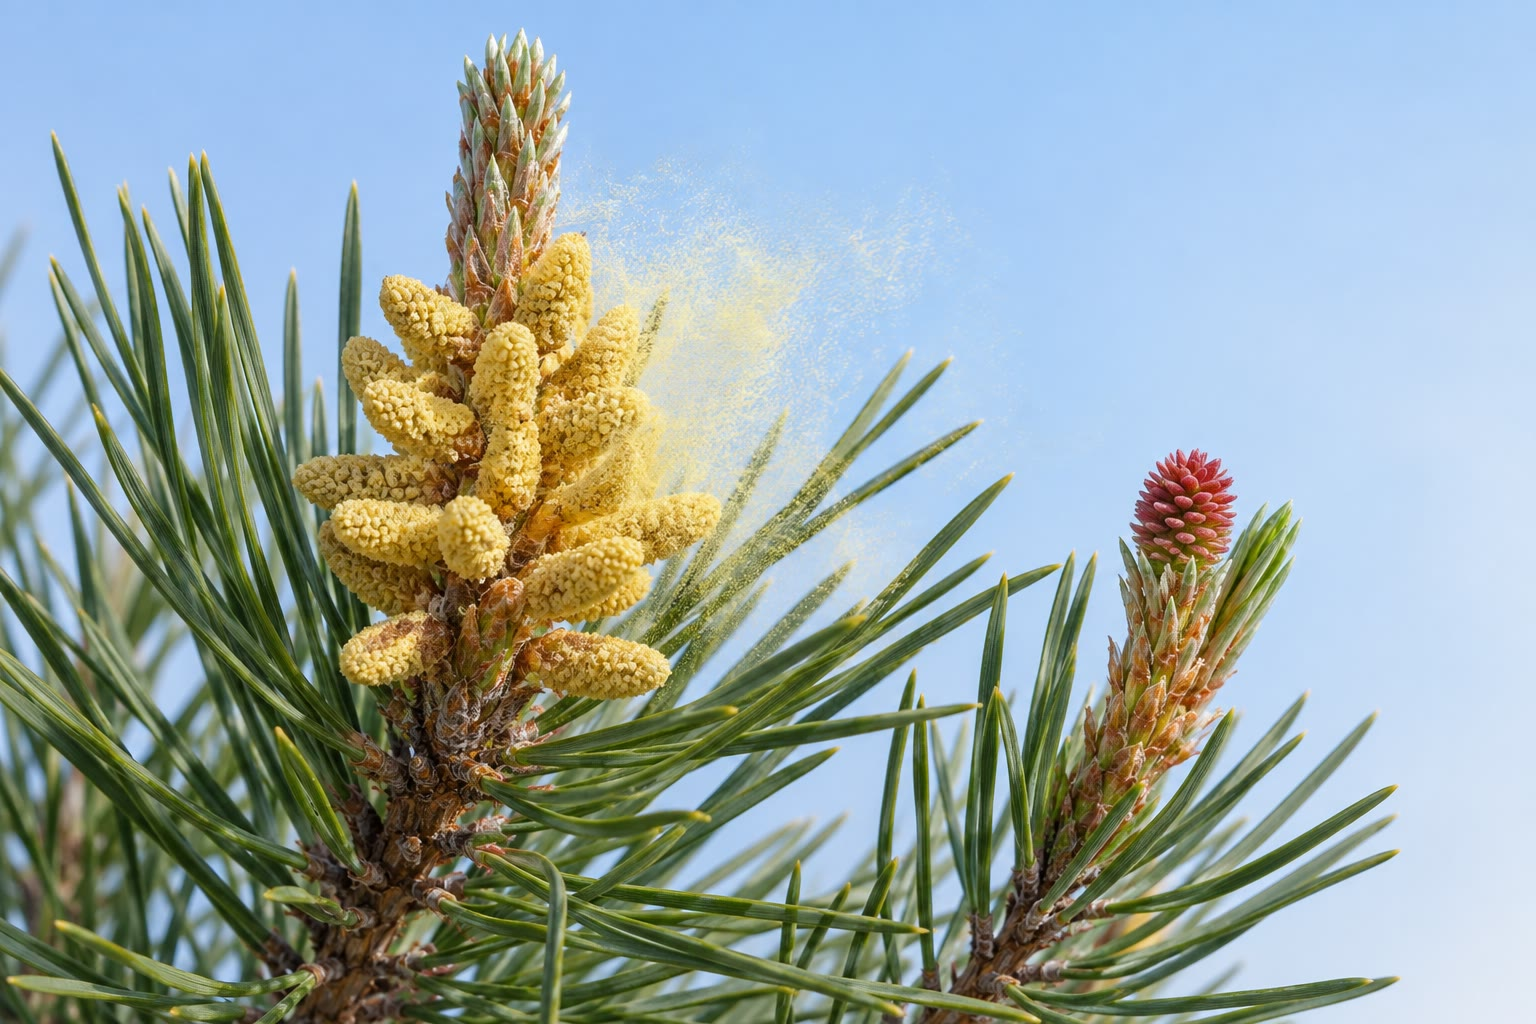
\includegraphics[width=0.6\linewidth]{images/book4/ai/b4-05-pine-cones.jpg}

{\small Sebuah pucuk pinus pada musim semi: segerombol runjung jantan
berwarna kuning yang melepaskan \omterm{def:b2:plant-life-cycles:heterospory}{serbuk sari}, dan sebuah runjung betina
merah kecil pada ujung pucuk lain, sisiknya terbuka untuk menangkapnya.}
\end{omfigure}

\begin{example}[Serbuk sari di dalam angin]\label{ex:b2:plant-life-cycles:pollen}
Sebutir \omterm{def:b2:plant-life-cycles:heterospory}{serbuk sari} pinus, selebar \qty{50}{\micro m} dengan dua
gelembung, jatuh pada kira-kira \qty{3}{cm/s}; sebatang pohon besar
melepaskan sekitar $10^{11}$ butir dalam satu musim, cukup untuk
menguningkan permukaan kolam. Peluang satu butirnya mendarat pada
sebuah \omterm{def:b2:plant-life-cycles:heterospory}{bakal biji} tertentu sangatlah kecil, dan siasatnya hanya
berhasil lewat jumlah: penyerbukan angin murah tiap butirnya, mahal
dalam jumlah butirnya, dan terbatas pada tumbuhan yang tumbuh dalam
rumpun sejenisnya --- konifer, rumput, ek. Tumbuhan berbunga
(\cref{ch:b2:angiosperm-reproduction}) menemukan cara mengantarkan
\omterm{def:b2:plant-life-cycles:heterospory}{serbuk sari} lewat hewan, satu butir sekaligus, ke alamat yang tepat.
\end{example}

\section{Kecenderungan menyeberangi tumbuhan darat}

\begin{proposition}[Empat kecenderungan]\label{prop:b2:plant-life-cycles:trends}
\index{penyusutan gametofit}
Dari \omterm{def:b2:plant-life-cycles:moss}{lumut} ke \omterm{def:b2:plant-life-cycles:fern}{tumbuhan paku} lalu ke tumbuhan berbiji: (1) \omterm{def:b2:plant-life-cycles:cycles}{sporofitnya}
tumbuh dari sebuah tangkai yang bergantung menjadi seluruh tumbuhannya,
dan \omterm{def:b2:plant-life-cycles:cycles}{gametofitnya} menyusut dari tumbuhannya menjadi sebuah sisik lalu
menjadi beberapa sel; (2) homospori berganti menjadi
\omterm{def:b2:plant-life-cycles:heterospory}{heterospori}, dan \omterm{def:b2:plant-life-cycles:cycles}{gametofit} betinanya tinggal pada tetuanya;
(3) pembuahannya beralih dari sperma yang berenang di dalam air
permukaan menjadi sebuah buluh \omterm{def:b2:plant-life-cycles:heterospory}{serbuk sari}, sehingga
perkembangbiakannya tidak lagi membutuhkan hujan; (4) satuan
penyebarannya beralih dari spora --- satu sel dengan cadangan sehari
--- menjadi biji, yaitu sebuah lembaga dengan makanan dan kulit, yang
dapat menunggu. Keturunan \omterm{def:b2:meiosis-heredity:meiosis}{diploidnya} diunggulkan di darat karena tubuh
\omterm{def:b2:meiosis-heredity:meiosis}{diploid} menutupi \omterm{def:b2:genome-diversification:mutation}{mutasi} \omterm{def:b2:meiosis-heredity:vocabulary}{resesif}, dapat tumbuh lebih besar dan lebih
panjang umur dengan sistem pembuluh, dan karena sebuah spora yang
dibuat secara \omterm{def:b2:meiosis-heredity:meiosis}{meiosis} pada \omterm{def:b2:plant-life-cycles:cycles}{sporofit} yang tinggi menempuh jarak lebih
jauh daripada gamet yang berenang dari \omterm{def:b2:plant-life-cycles:cycles}{gametofit} yang rendah.
Kecenderungan itu berlanjut sampai ke tumbuhan berbunga, tempat
\omterm{def:b2:plant-life-cycles:cycles}{gametofit} betinanya tinggal tujuh sel dan bijinya terbungkus sebuah
buah.
\end{proposition}

\begin{example}[Perbandingan kelompoknya]\label{ex:b2:plant-life-cycles:table}
\begin{center}
\small
\begin{tabular}{p{2.3cm}p{3.1cm}p{3.1cm}p{3.3cm}}
\hline
 & \omterm{def:b2:plant-life-cycles:moss}{lumut} & \omterm{def:b2:plant-life-cycles:fern}{tumbuhan paku} & konifer \\
\hline
keturunan yang \omterm{def:b2:meiosis-heredity:vocabulary}{dominan} & \omterm{def:b2:plant-life-cycles:cycles}{gametofit} & \omterm{def:b2:plant-life-cycles:cycles}{sporofit} & \omterm{def:b2:plant-life-cycles:cycles}{sporofit} \\
\omterm{def:b2:plant-life-cycles:cycles}{gametofit} & pucuk berdaun, cm & \omterm{def:b2:plant-life-cycles:fern}{protalus}, mm, dan bebas
  & butir \omterm{def:b2:plant-life-cycles:heterospory}{serbuk sari} (4 sel); isi \omterm{def:b2:plant-life-cycles:heterospory}{bakal bijinya} (ribuan sel) \\
spora & satu macam & satu macam & \omterm{def:b2:plant-life-cycles:heterospory}{mikrospora}, \omterm{def:b2:plant-life-cycles:heterospory}{megaspora} \\
pembuahan & sperma berenang di air & sperma berenang di air & buluh \omterm{def:b2:plant-life-cycles:heterospory}{serbuk sari} \\
satuan penyebaran & spora & spora & biji \\
jaringan pembuluh & tidak ada & xilem, floem & xilem, floem, kayu \\
\hline
\end{tabular}
\end{center}
\end{example}

\section{Latihan}

\begin{exercise}[$\star$]\label{exo:b2:plant-life-cycles:1}
Definisikan \omterm{def:b2:plant-life-cycles:cycles}{gametofit}, \omterm{def:b2:plant-life-cycles:cycles}{sporofit}, spora, dan gamet, lalu katakan dengan
pembelahan macam apa (mitosis atau \omterm{def:b2:meiosis-heredity:meiosis}{meiosis}) masing-masing dihasilkan.
\end{exercise}

\begin{exercise}[$\star$]\label{exo:b2:plant-life-cycles:2}
\omterm{def:b2:plant-life-cycles:fern}{Tumbuhan paku} \emph{Ophioglossum reticulatum} memiliki \num{1260}
kromosom di dalam sel daunnya. Berapa banyak di dalam sebuah spora,
sebuah sel \omterm{def:b2:plant-life-cycles:fern}{protalus}, sebuah sperma, sebuah sel telur, sebuah zigot?
\end{exercise}

\begin{exercise}[$\star$]\label{exo:b2:plant-life-cycles:3}
Keturunan mana yang merupakan bantalan hijau sebatang \omterm{def:b2:plant-life-cycles:moss}{lumut}? Tangkai
cokelat berkapsulnya? Sehelai ental paku? Sebuah \omterm{def:b2:plant-life-cycles:fern}{protalus}? Sebutir
\omterm{def:b2:plant-life-cycles:heterospory}{serbuk sari}? Simpanan makanan sebutir biji pinus? Lembaga biji pinus?
\end{exercise}

\begin{exercise}[$\star$]\label{exo:b2:plant-life-cycles:4}
Sebutkan ketiga macam \omterm{def:b2:plant-life-cycles:cycles}{daur hidupnya} dan berikan sebuah organisme bagi
masing-masing. Di manakah \omterm{def:b2:meiosis-heredity:meiosis}{meiosis} berlangsung pada tiap daurnya?
\end{exercise}

\begin{exercise}[$\star\star$]\label{exo:b2:plant-life-cycles:5}
Sperma \omterm{def:b2:plant-life-cycles:moss}{lumut} berenang pada \qty{100}{\micro m/s}. Berapa lama ia
mencapai sebuah \omterm{def:b2:plant-life-cycles:moss}{arkegonium} sejauh \qty{3}{cm}? Selaput embun menguap
dalam \qty{20}{min} sesudah matahari terbit: berapakah jangkauan
maksimal pembuahannya? Ulaslah ukuran koloni \omterm{def:b2:plant-life-cycles:moss}{lumutnya}.
\end{exercise}

\begin{exercise}[$\star\star$]\label{exo:b2:plant-life-cycles:6}
Hitunglah kelajuan pengendapan di udara sebuah spora paku berjari-jari
\qty{15}{\micro m} dan bermassa jenis \qty{1100}{kg/m^3} ($\eta =
\qty{1.8e-5}{Pa.s}$, $\rho_{\text{udara}} = \qty{1.2}{kg/m^3}$), serta
jarak yang ditempuhnya dari \qty{0.5}{m} di dalam angin \qty{2}{m/s}.
Ulangi bagi sebutir biji pinus bermassa \qty{5}{mg} yang sayapnya
memberinya kelajuan turun \qty{0.8}{m/s}, dilepaskan dari \qty{20}{m}.
\end{exercise}

\begin{exercise}[$\star\star$]\label{exo:b2:plant-life-cycles:7}
Sehelai ental paku mengusung \num{200} \omterm{def:b2:plant-life-cycles:fern}{sorus} berisi \num{40}
\omterm{def:b2:plant-life-cycles:fern}{sporangium}, dan tiap \omterm{def:b2:plant-life-cycles:fern}{sporangium} membuat \num{64} spora. Berapa spora
tiap entalnya? Kalau satu spora dari tiap $10^{5}$ menjadi sebuah
\omterm{def:b2:plant-life-cycles:fern}{protalus} dan satu \omterm{def:b2:plant-life-cycles:fern}{protalus} dari tiap \num{50} menghasilkan sebuah
\omterm{def:b2:plant-life-cycles:cycles}{sporofit}, berapa \omterm{def:b2:plant-life-cycles:fern}{tumbuhan paku} muda yang dihasilkan sehelai ental?
\end{exercise}

\begin{exercise}[$\star\star$]\label{exo:b2:plant-life-cycles:8}
Jelaskan mengapa \omterm{def:b2:plant-life-cycles:heterospory}{heterospori} adalah prasyarat bagi biji, dan mengapa
tumbuhan homospor tidak dapat mengurung \omterm{def:b2:plant-life-cycles:cycles}{gametofit} betinanya di dalam
sebuah \omterm{def:b2:plant-life-cycles:heterospory}{bakal biji}.
\end{exercise}

\begin{exercise}[$\star\star$]\label{exo:b2:plant-life-cycles:9}
Bandingkanlah sebuah spora paku (bola berjari-jari \qty{15}{\micro m},
bermassa jenis \qty{1100}{kg/m^3}) dan sebutir biji pinus
(\qty{5}{mg}) sebagai satuan penyebaran: massanya, kandungan energinya
(ambillah \qty{20}{kJ/g} bahan kering, \qty{50}{\%} kering), dan apa
yang dapat dan tidak dapat dikerjakan masing-masing saat mendarat.
\end{exercise}

\begin{exercise}[$\star\star\star$]\label{exo:b2:plant-life-cycles:10}
Sebatang pinus melepaskan $10^{11}$ butir \omterm{def:b2:plant-life-cycles:heterospory}{serbuk sari} di atas sebuah
hutan; pada ketinggian \omterm{def:b2:plant-life-cycles:heterospory}{bakal bijinya}, butirnya tersebar di dalam
lapisan setebal \qty{20}{m} di atas \qty{1}{km^2}. Taksirlah kepekatan
\omterm{def:b2:plant-life-cycles:heterospory}{serbuk sarinya} (butir tiap meter kubik), cacah butir tiap sekon yang
melewati bukaan mikropil sebuah \omterm{def:b2:plant-life-cycles:heterospory}{bakal biji} (\qty{0.1}{mm^2}) di dalam
angin \qty{2}{m/s}, dan waktu bagi sebuah \omterm{def:b2:plant-life-cycles:heterospory}{bakal biji} untuk menerima
satu butir. Apa yang dikatakannya tentang waktu pembukaan runjungnya?
\end{exercise}

\begin{exercise}[$\star\star\star$]\label{exo:b2:plant-life-cycles:11}
Berikan tiga alasan mengapa keturunan \omterm{def:b2:meiosis-heredity:meiosis}{diploid} akhirnya mendominasi
\omterm{def:b2:plant-life-cycles:cycles}{daur hidup} tumbuhan darat, dan satu alasan mengapa keturunan \omterm{def:b2:meiosis-heredity:meiosis}{haploidnya}
tidak lenyap sama sekali.
\end{exercise}

\begin{exercise}[$\star\star\star$]\label{exo:b2:plant-life-cycles:12}
Hofmeister bekerja sebelum kromosom dikenal. Jelaskan apa yang dapat
dan tidak dapat ditetapkannya tentang \omterm{def:b2:plant-life-cycles:cycles}{pergiliran keturunan}
lewat mikroskopi dan pembiakan semata, serta apa yang ditambahkan
cacah kromosomnya.
\end{exercise}

\section{Soal: Dari Spora ke Biji}

\begin{problem}[{Soal akhir pekan --- aritmetika perkembangbiakan
sebatang tumbuhan paku dan sebatang pinus dibandingkan, dari cacah
spora dan butir serbuk sarinya sampai penyebarannya, nasib gametofitnya,
dan ongkos sebutir biji, berakhir pada cacah propagul yang harus dibuat
tiap tumbuhan demi satu penggantinya}]
\label{pb:b2:plant-life-cycles:1}
Sebatang \omterm{def:b2:plant-life-cycles:fern}{tumbuhan paku} mengusung \num{10} ental subur, masing-masing
dengan \num{200} \omterm{def:b2:plant-life-cycles:fern}{sorus} berisi \num{40} \omterm{def:b2:plant-life-cycles:fern}{sporangium} yang membuat
\num{64} spora. Sporanya: jari-jari \qty{15}{\micro m}, massa jenis
\qty{1100}{kg/m^3}. Sebatang pinus menghasilkan \omterm{def:b2:plant-life-cycles:heterospory}{bakal biji} senilai
$2\times 10^{4}$ runjung betina sepanjang hidupnya --- ambillah
\num{100} \omterm{def:b2:plant-life-cycles:heterospory}{bakal biji} tiap runjung --- dan $10^{11}$ butir \omterm{def:b2:plant-life-cycles:heterospory}{serbuk sari}
tiap tahun. Bijinya: \qty{5}{mg}, \qty{50}{\%} bahan kering pada
\qty{20}{kJ/g}. Udaranya: $\eta = \qty{1.8e-5}{Pa.s}$, $\rho =
\qty{1.2}{kg/m^3}$; $g = \qty{9.81}{m/s^2}$.

\medskip
\noindent\textbf{Bagian I --- Spora pakunya.}
\begin{enumerate}
  \item Hitunglah cacah spora yang dilepaskan tumbuhannya dalam satu
        musim.
  \item Hitunglah massa satu spora dan massa seluruh panennya.
  \item Hitunglah kelajuan pengendapan sporanya di udara.
  \item Dari ental pada \qty{0.5}{m} di dalam angin \qty{1.5}{m/s},
        seberapa jauh sporanya menempuh? Di atas daerah seluas apa
        (sebuah cakram berjari-jari itu) sporanya tersebar, dan berapa
        banyak yang mendarat tiap meter persegi?
  \item Jelaskan mengapa olakan membawa beberapa sporanya jauh lebih
        jauh, dan apa artinya bagi penjajahan sebuah pulau baru.
  \item Hitunglah kandungan energi satu spora (\qty{50}{\%} bahan
        kering pada \qty{20}{kJ/g}) dan kandungan energi seluruh
        panennya, lalu bandingkan dengan energi sebutir biji pinus.
\end{enumerate}

\medskip
\noindent\textbf{Bagian II --- \omterm{def:b2:plant-life-cycles:cycles}{Gametofitnya}.}
Satu spora dari tiap $2\times 10^{4}$ mendarat di tanah yang cukup
lembap untuk tumbuh menjadi sebuah \omterm{def:b2:plant-life-cycles:fern}{protalus}; sebuah \omterm{def:b2:plant-life-cycles:fern}{protalus} hidup
\num{6} pekan dan membutuhkan satu malam yang basah --- berpeluang
$0.2$ tiap pekan --- untuk pembuahan; sebuah \omterm{def:b2:plant-life-cycles:fern}{protalus} yang telah
dibuahi memberi sebuah \omterm{def:b2:plant-life-cycles:cycles}{sporofit} muda dengan peluang $0.5$; sebuah
\omterm{def:b2:plant-life-cycles:cycles}{sporofit} muda bertahan sampai dewasa dengan peluang $0.02$.
\begin{enumerate}[resume]
  \item Berapa banyak \omterm{def:b2:plant-life-cycles:fern}{protalus} yang dihasilkan panen tumbuhannya?
  \item Hitunglah peluang bahwa sebuah \omterm{def:b2:plant-life-cycles:fern}{protalus} mengalami sedikitnya
        satu malam yang basah dalam enam pekannya.
  \item Hitunglah harapan cacah \omterm{def:b2:plant-life-cycles:fern}{tumbuhan paku} dewasa yang dihasilkan
        panen satu musim.
  \item Kalau tetuanya hidup \num{30} tahun, berapa keturunan dewasa
        yang ditinggalkannya, dan apa artinya bagi populasi
        \omterm{def:b2:plant-life-cycles:fern}{tumbuhan pakunya}?
  \item Sperma paku berenang pada \qty{100}{\micro m/s} dan \omterm{def:b2:plant-life-cycles:moss}{arkegonium}
        sebuah \omterm{def:b2:plant-life-cycles:fern}{protalus} terletak \qty{1}{mm} dari \omterm{def:b2:plant-life-cycles:moss}{anteridiumnya}
        sendiri. Berapa lama pembuahan sendirinya berlangsung? Mengapa
        banyak \omterm{def:b2:plant-life-cycles:fern}{tumbuhan paku} tetap menghindarinya (berikan satu
        mekanisme)?
  \item Dalam arti apa \omterm{def:b2:plant-life-cycles:fern}{protalusnya} adalah mata rantai terlemah daur
        pakunya?
\end{enumerate}

\medskip
\noindent\textbf{Bagian III --- \omterm{def:b2:plant-life-cycles:heterospory}{Serbuk sari} pinusnya.}
\begin{enumerate}[resume]
  \item Sebutir \omterm{def:b2:plant-life-cycles:heterospory}{serbuk sari} adalah bola berjari-jari \qty{25}{\micro m}
        dengan massa jenis efektif \qty{600}{kg/m^3} (gelembung
        udaranya sudah diperhitungkan). Hitunglah kelajuan
        pengendapannya.
  \item Dari sebuah runjung pada \qty{15}{m} di dalam angin
        \qty{3}{m/s}, seberapa jauh ia menempuh?
  \item Sejumlah $10^{11}$ butirnya tersebar di dalam \qty{1}{km^2}
        hutan sampai kedalaman \qty{20}{m}. Hitunglah kepekatannya.
  \item Sebuah mikropil menyajikan bukaan seluas \qty{0.1}{mm^2}
        kepada angin \qty{2}{m/s}. Hitunglah cacah butir yang
        memasukinya tiap jam, dan waktu untuk menerima butir pertamanya.
  \item Jelaskan mengapa sebatang pinus tunggal sejauh \qty{5}{km} dari
        hutannya hampir tidak menghasilkan biji, dan mengapa spesies
        yang diserbuki angin tumbuh dalam rumpun.
  \item Bandingkanlah angkanya: berapa butir \omterm{def:b2:plant-life-cycles:heterospory}{serbuk sari} yang dibuat
        hutannya tiap \omterm{def:b2:plant-life-cycles:heterospory}{bakal biji}, kalau hutannya memuat \num{1000}
        pinus dengan masing-masing \num{2000} \omterm{def:b2:plant-life-cycles:heterospory}{bakal biji}?
\end{enumerate}

\medskip
\noindent\textbf{Bagian IV --- Biji pinusnya.}
Dari \omterm{def:b2:plant-life-cycles:heterospory}{bakal biji} pohonnya, \qty{60}{\%} diserbuki dan \qty{80}{\%} di
antaranya mengisi sebutir biji; sebutir biji menjadi kecambah dengan
peluang $0.05$ dan sebuah kecambah menjadi dewasa dengan peluang $0.01$.
\begin{enumerate}[resume]
  \item Hitunglah cacah biji yang dibuat pohonnya sepanjang hidupnya,
        serta massa dan energi keseluruhannya.
  \item Sebutir biji bersayap turun pada \qty{0.8}{m/s}. Dari
        \qty{20}{m} di dalam angin \qty{3}{m/s}, seberapa jauh ia
        menempuh? Bandingkan dengan \omterm{def:b2:plant-life-cycles:heterospory}{serbuk sarinya}.
  \item Hitunglah harapan cacah keturunan dewasanya, lalu bandingkan
        dengan keturunan \omterm{def:b2:plant-life-cycles:fern}{tumbuhan pakunya}.
  \item Hitunglah energi yang ditanamkan pohonnya tiap keturunan
        dewasa, dan energi \omterm{def:b2:plant-life-cycles:fern}{tumbuhan pakunya} tiap keturunan dewasa
        (sporanya saja), lalu bandingkan.
  \item Spora paku dapat menunggu beberapa pekan; biji pinus beberapa
        tahun. Jelaskan, dengan angka energinya, mengapa bijinya
        sanggup berdorman dan sporanya tidak.
  \item Berikan dua keuntungan yang membuat bijinya sepadan dengan
        ongkosnya dan dua keadaan yang membuat siasat \omterm{def:b2:plant-life-cycles:fern}{tumbuhan pakunya}
        lebih baik.
  \item Nyatakan hasilnya: propagul tiap keturunan dewasa bagi
        \omterm{def:b2:plant-life-cycles:fern}{tumbuhan paku} dan bagi pinusnya, serta energi yang dibelanjakan
        masing-masing tiap keturunan dewasa.
\end{enumerate}
\end{problem}
